 
\setlength{\parindent}{0cm}
\newpage
\maketitle
\newpage
\pgfplotsset{every tick label/.append style={font=\tiny\sffamily}} 


\begin{tikzpicture}[
    triangle/.style = {regular polygon, 
                       regular polygon sides=3, 
	               minimum size=0.3cm,
                       isosceles triangle, 
                       isosceles triangle apex angle=90, 
	               anchor=apex,
	               color=black!30,
                       rotate=-45 },
    box/.style = {      
                       draw,
		       inner sep=0pt,
	               color=black!50,
		       anchor=south east,
		       minimum size=0.09cm}
   ]
   
   \node [rectangle] at (-1,6.5) {};
   \node [anchor=west] at (-1,4) {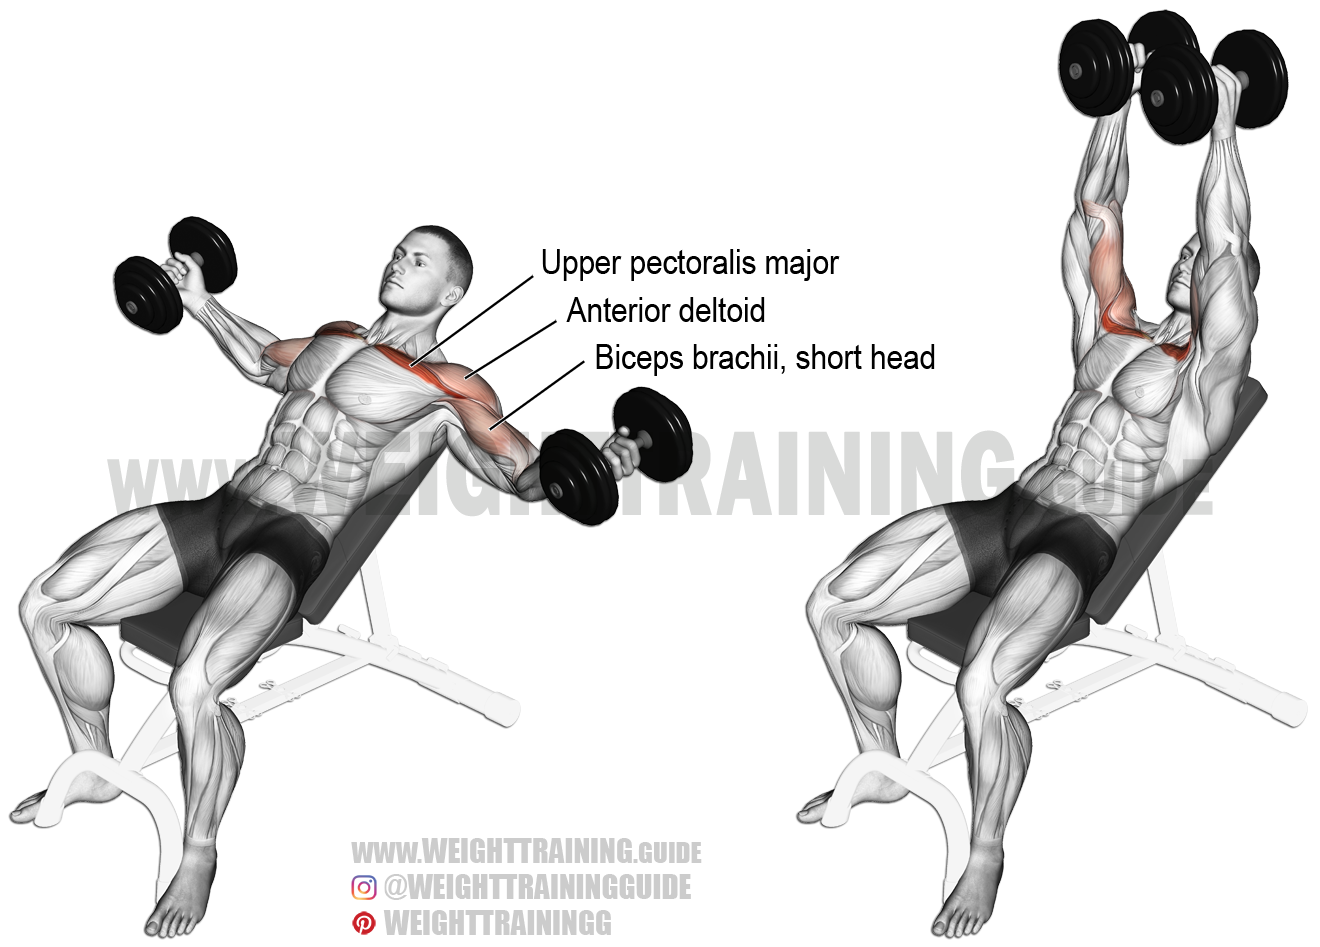
\includegraphics[height=4cm]{./incline-dumbbell-fly.png}};
   \node [anchor=west] at (-1,6) {\textsf{\Large Incline dumbbell fly}};

   \node at  (-0.5,1.25)  [anchor=east]{\tiny\textsf{mnt}};
   \node at  (-0.5,0.75)  [anchor=east]{\tiny\textsf{day}};
    \node at (-0.5,0.25)  [anchor=east]{\tiny\textsf{wu}};
    \node at (-0.5,-0.25) [anchor=east]{\tiny\textsf{r1}};
    \node at (-0.5,-0.75) [anchor=east]{\tiny\textsf{r2}};
    \node at (-0.5,-1.25) [anchor=east]{\tiny\textsf{r3}};
    \node at (-0.5,-1.75) [anchor=east]{\tiny\textsf{r4}};

    \foreach \x in {1,...,2} {
    \foreach \y in {0,...,17} {
	 \draw (\y/2, \x/2) -- ++ (-.5,0);
	 \draw (\y/2, \x/2) -- ++ (0,0.1);
    }
    }

    \foreach \x in {0,...,4} {
    \foreach \y in {0,...,17} {
         \node [draw,triangle] at (\y/2,-\x/2) {};
         \node [draw, box] at (\y/2,-\x/2) {};
    }
    }

   \node at  (4,-2.35)  {\footnotesize\textsf{MAX}};
   \node at  (4,-4.85)  {\footnotesize\textsf{1RM}};

  \begin{axis}[
          every axis/.append style={font=\tiny},
          grid style={gray!20},
          major y grid style=black,
          minor grid style=gray!20,
          grid=both,
          width=10.58cm,
          height=3.5cm,
          ymin=4,
          ymax=20,
          xmax=19,
          xmin=1,
          xticklabel=\empty,
          minor x tick num=1,
          minor y tick num=4,
          at={(-.5cm,-4.5cm)},
          ]
  \end{axis}

  \begin{axis}[
          every axis/.append style={font=\tiny},
          grid style={gray!20},
          major y grid style=black,
          minor grid style=gray!20,
          grid=both,
          width=10.58cm,
          height=3.5cm,
          ymin=4,
          ymax=12,
          xmax=19,
          xmin=1,
          xticklabel=\empty,
          minor x tick num=1,
          minor y tick num=4,
          at={(-.5cm,-7cm)},
          ]
   \end{axis}
\end{tikzpicture}
\newpage
\begin{tikzpicture}[
    triangle/.style = {regular polygon, 
                       regular polygon sides=3, 
	               minimum size=0.3cm,
                       isosceles triangle, 
                       isosceles triangle apex angle=90, 
	               anchor=apex,
	               color=black!30,
                       rotate=-45 },
    box/.style = {      
                       draw,
		       inner sep=0pt,
	               color=black!50,
		       anchor=south east,
		       minimum size=0.09cm}
   ]
   
   \node [rectangle] at (-1,6.5) {};

   \node at (-0.5, 6) [anchor=east] {\tiny\textsf{SRmin}};
   \node at (-0.5, 6) [anchor=west, text width=10cm, inner sep=0pt, align=left] { \tiny 10 };

   \node at (-0.5, 5.7) [anchor=east] {\tiny\textsf{SRmax}};
   \node at (-0.5, 5.7) [anchor=west, text width=10cm, inner sep=0pt, align=left] { \tiny 20 };

   \node at (-0.5, 5.4) [anchor=east] {\tiny\textsf{notes}};
   \node at (-0.5, 5.4) [anchor=west, text width=10cm, inner sep=0pt, align=left] { \begin{minipage}{0.50\textwidth} \tiny weight is the weight of a single dumbbell \end{minipage} };



   \node at (-0.5,1.25)  [anchor=east] {\tiny\textsf{mnt}};
   \node at (-0.5,0.75)  [anchor=east] {\tiny\textsf{day}};
   \node at (-0.5,0.25)  [anchor=east] {\tiny\textsf{wu}};
   \node at (-0.5,-0.25) [anchor=east] {\tiny\textsf{r1}};
   \node at (-0.5,-0.75) [anchor=east] {\tiny\textsf{r2}};
   \node at (-0.5,-1.25) [anchor=east] {\tiny\textsf{r3}};
   \node at (-0.5,-1.75) [anchor=east] {\tiny\textsf{r4}};

    \foreach \x in {1,...,2} {
    \foreach \y in {0,...,17} {
	 \draw (\y/2, \x/2) -- ++ (-.5,0);
	 \draw (\y/2, \x/2) -- ++ (0,0.1);
    }
    }

    \foreach \x in {0,...,4} {
    \foreach \y in {0,...,17} {
         \node [draw,triangle] at (\y/2,-\x/2) {};
         \node [draw, box] at (\y/2,-\x/2) {};
    }
    }

  \begin{axis}[
          every axis/.append style={font=\tiny},
          grid style={gray!20},
          major y grid style=black,
          minor grid style=gray!20,
          grid=both,
          width=10.58cm,
          height=3.5cm,
          ymin=4,
          ymax=20,
          xmax=19,
          xmin=1,
          xticklabel=\empty,
          minor x tick num=1,
          minor y tick num=4,
          at={(-.5cm,-4.5cm)},
          ]
  \end{axis}

  \begin{axis}[
          every axis/.append style={font=\tiny},
          grid style={gray!20},
          major y grid style=black,
          minor grid style=gray!20,
          grid=both,
          width=10.58cm,
          height=3.5cm,
          ymin=4,
          ymax=12,
          xmax=19,
          xmin=1,
          xticklabel=\empty,
          minor x tick num=1,
          minor y tick num=4,
          at={(-.5cm,-7cm)},
          ]
   \end{axis}
\end{tikzpicture}
